\RequiredExercise{CSS Layout Grundlagen}
%
\par Verwenden Sie als Grundlage Aufgabe 6 von Blatt 2. Sollten Sie diese nicht
durchgeführt haben, so laden Sie sich die Lösung aus dem Internet herunter:
%
\begin{figure}[!h]
\centering
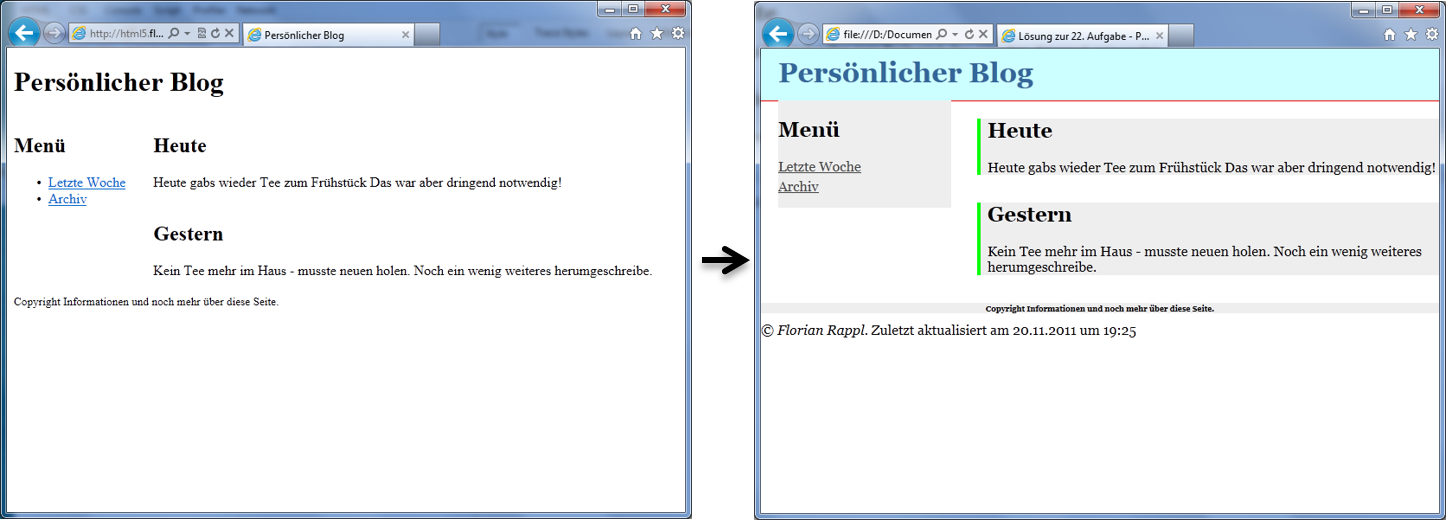
\includegraphics[width=1\textwidth]{Exercises/Figures/applycss.png}
\caption{Grau markiert sind die Bereiche der einzelnen Boxen}
\label{fig:applycss}
\end{figure}
%
\par Verwandeln Sie diese Seite durch CSS Code in das gezeigte Layout. Wichtig
sind hierbei folgende Details:
%
\begin{itemize}
\item
Die Seite soll die volle Fensterbreite ausnutzen.
\item
Der gesamte Text soll in der Schriftart \emph{Georgia} mit einer Schriftgröße
von \qty{12}{pt} angezeigt werden.
\item
Der Titel der Seite soll nach unten hin durch einen \qty{1}{px} Rahmen und
blaue Schrift abgegrenzt sein.
\item
Das Menü soll eine feste Breite von \qty{200}{px} und genau wie der Titel
\qty{10}{px} Abstand nach links besitzen. Die Liste für das Menü soll keinen
Listenstil haben.
\item
Die Artikel sollen \qty{30}{px} Abstand zum Menü und einen linken Rahmen
haben. Jeder Artikel soll einen Abstand nach unten von \qty{2}{em} besitzen.
\item
Die Copyright-Information soll fett, in einer Schriftgröße von \qty{8}{pt} und
horizontal in der Mitte der Seite (unterhalb des gesamten Inhalts) angezeigt
werden. 
\item
Es dürfen keine fließenden Elemente, d.h.
%
\begin{lstlisting}
float: left; //oder
float: right;
\end{lstlisting}
%
verwendet werden.
\end{itemize}